\documentclass[11pt]{amsbook}

\usepackage[turkish]{babel}

\usepackage{../Ceyhun}
\usepackage{../amsTurkish}

\begin{document}

    \hPage{065}

    \subsection{ÇİZGİLER ARASINDA İŞLEMLER}
    
    İki ayrı çizge arasındaki işlemleri tanımlamadan önce bir çizge ile kendi arasında tanımlanan işlemleri inceleyelim.
    
    \begin{definition}
        Ç ve $Ç^n$, düğüm kümeleri arasında 1:1 karşıdüşme olan 2 çizgeyi göstersin.Ç de
        \begin{align*}
            1 \leq u(d'_{i},d'_{j}) \leq n
        \end{align*}
        
        \hfill\begin{minipage}{\dimexpr\textwidth-18mm}
        eşitsizliğinin sağlandığı her $d_{i},d_{j}\in\Delta$ düğüm çifti arasında $Ç^n$ de de bir ayrıt varsa, $Ç^n$ ,Ç nin n ninci \underline{kuvvet}idir. 
        \xdef\tpd{\the\prevdepth}
        \end{minipage} 
        
    \end{definition}
    
    Bu tanıma göre, Şekil 2.3.la daki çizgenin ikinci kuvveti, Şekil 2.3.1b de olduğu gibi bulunabilir. Ç de $u(1,4)=3>2$ olduğu için, $Ç^2$ de bu düğümler arasında bir ayrıt yoktur.
    
    
    \begin{table}[ht]
        \begin{tabular}{l@{\hskip 1.5in}c@{\hskip 0.5in}c}
            \item[c)] Ç
            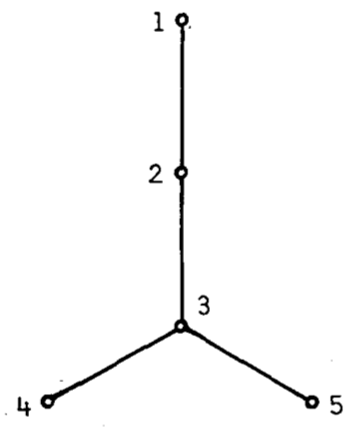
\includegraphics[width=1.4in]{images/ceyhun-065-fig01.png} &
            \item[c)] $Ç^2$
            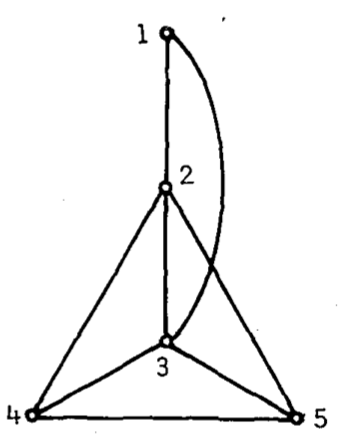
\includegraphics[width=1.4in]{images/ceyhun-065-fig02.png}
        \end{tabular}
    \end{table}
    
    Şekil 2.3.1 Ç ve $Ç^2$ çizgeleri.

\end{document}